\chapter{实验结果}
\label{cha:result}

\section{数据集的准备 \label{section:mypre}}
在第 \ref{section:pointsetgenpre} 节中,我们介绍了 PointSetGen
使用 RenderForCNN\cite{rendercnn} 的方法,通过计算机图形学中的渲染手段,获取图像训练数据。
但通过观察 PointSetGen 的实现,我们发现了其数据集的准备工作有一定的不足:
\begin{itemize}
	\item 仰角与距离固定:渲染时固定了摄像机的仰角为 $20^\circ$,%摄像机
	      到物体的距离为 $2.5$ 倍物体半径。这使得 PointSetGen 不能适应新的摄像机视角与距离;
	\item 标注与视角相关:标注的真实点云数据是相对于相机坐标系的。这会使得标注点云随着摄像机视角的旋转而转动。
	      由于网络的核心任务是重建而非视角估计,因此,这样的转动在一定程度上是噪音,不利于网络把握三维模型在几何形状上的规律;
	\item 模型视角少:每个模型渲染的视角数较少,没有充分利用已有数据的信息;
	\item 背景色固定:渲染出的图像中,背景色的不透明度 (Alpha) 通道被设为了 0,但颜色 (RGB) 通道 被设为了固定常数。此处的 RGB 值虽然没有意义,但它仍然参与了网络的计算,影响着输出结果。
\end{itemize}
对此,我们使用如下的新策略,重新对 ShapeNet\cite{shapenet} 进行了渲染,从而完成了数据集的准备工作:
\begin{itemize}
	\item 视角随机化:使得摄像机的仰角从 $20^\circ$ 到 $60^\circ$ 间均匀分布,方向角从 $0^\circ$ 到 $360^\circ$ 间均匀分布,因为这基本上涵盖了人类摄影的常见角度;

	\item 距离随机化:使得摄像机到物体的距离从 $1.7$ 倍物体半径到 $2.5$ 倍物体半径间均匀分布。过远或者过近会使得物体过大或者过小,不利于重建;

	\item 光照随机化:引入 3 到 10 个不等的点光源,其位置、亮度均随机,用于模拟各种强弱光环境;

	\item 标注与视角无关:标注的真实点云数据使用局部坐标系,其不会随着视角的变化而转动,利于网络
	      %的
	      学习出三维模型的几何分布规律;

	\item 多视角渲染:每个模型渲染 100 个不同的视角,充分挖掘已有的数据;

	\item 背景色随机化:背景色设置为 Alpha 通道为 0,但 RGB 通道为随机值的颜色。
	      这使得网络的输出尽可能不受背景色 RGB 值的影响。
\end{itemize}

表格 \ref{tab:render} 展示了 PointSetGen 所渲染的数据集与本工作所渲染的数据集的差别。
可以看到,与 PointSetGen 相比,本工作渲染的数据集质量更高,视角更多,光照变化也更丰富,
具更适合做为训练网络的数据。

\begin{table}[htb]
	\centering
	\caption{PointSetGen\cite{pointsetgen} 与 本工作渲染的数据集(部分)\label{tab:render}}
	\begin{tabularx}{\linewidth}{ccc}
		\toprule[1.5pt]
		{\heiti PSG\cite{pointsetgen}}                     &  & {\heiti 本工作}
		\\\midrule[1pt]
		{\includegraphics[width=.145\textwidth]{data/1/a}} &  &
		{\includegraphics[width=.145\textwidth]{data/1/1}}
			{\includegraphics[width=.145\textwidth]{data/1/2}}
			{\includegraphics[width=.145\textwidth]{data/1/3}}
			{\includegraphics[width=.145\textwidth]{data/1/4}}
			{\includegraphics[width=.145\textwidth]{data/1/5}}
		\\
		{\includegraphics[width=.145\textwidth]{data/2/a}} &  &
		{\includegraphics[width=.145\textwidth]{data/2/1}}
			{\includegraphics[width=.145\textwidth]{data/2/2}}
			{\includegraphics[width=.145\textwidth]{data/2/3}}
			{\includegraphics[width=.145\textwidth]{data/2/4}}
			{\includegraphics[width=.145\textwidth]{data/2/5}}
		\\
		{\includegraphics[width=.145\textwidth]{data/3/a}} &  &
		{\includegraphics[width=.145\textwidth]{data/3/1}}
			{\includegraphics[width=.145\textwidth]{data/3/2}}
			{\includegraphics[width=.145\textwidth]{data/3/3}}
			{\includegraphics[width=.145\textwidth]{data/3/4}}
			{\includegraphics[width=.145\textwidth]{data/3/5}}
		\\
		{\includegraphics[width=.145\textwidth]{data/4/a}} &  &
		{\includegraphics[width=.145\textwidth]{data/4/1}}
			{\includegraphics[width=.145\textwidth]{data/4/2}}
			{\includegraphics[width=.145\textwidth]{data/4/3}}
			{\includegraphics[width=.145\textwidth]{data/4/4}}
			{\includegraphics[width=.145\textwidth]{data/4/5}}
		\\
		{\includegraphics[width=.145\textwidth]{data/5/a}} &  &
		{\includegraphics[width=.145\textwidth]{data/5/1}}
			{\includegraphics[width=.145\textwidth]{data/5/2}}
			{\includegraphics[width=.145\textwidth]{data/5/3}}
			{\includegraphics[width=.145\textwidth]{data/5/4}}
			{\includegraphics[width=.145\textwidth]{data/5/5}}
		\\
		\bottomrule[1.5pt]
	\end{tabularx}
\end{table}


% 实验结果

% Mask 表现

\section{Mask 提取与三维重建结果}
为了分别展现各个模块的质量,在本节中我们暂时假设:对于重建任务,算法已经得到了精确的 mask。
\subsection{Mask 提取\label{section:mask}}
正如第 \ref{my:mask} 节中所介绍的,我们希望手动标注各种大物体的 mask,作为训练数据集和测试数据集,对 Mask R-CNN 做迁移学习的训练。

然而标注 mask 任务通常很繁杂。由于时间有限,因此我们仅仅对少量的物体进行了测试。

迁移学习前后,模型给出的 mask 如图 \ref{fig:transferchange} 所示。可以看到,通过迁移学习,mask 的质量有了很大的提升。
\begin{figure}[h]
	\centering%
	\subcaptionbox{迁移学习前}
	{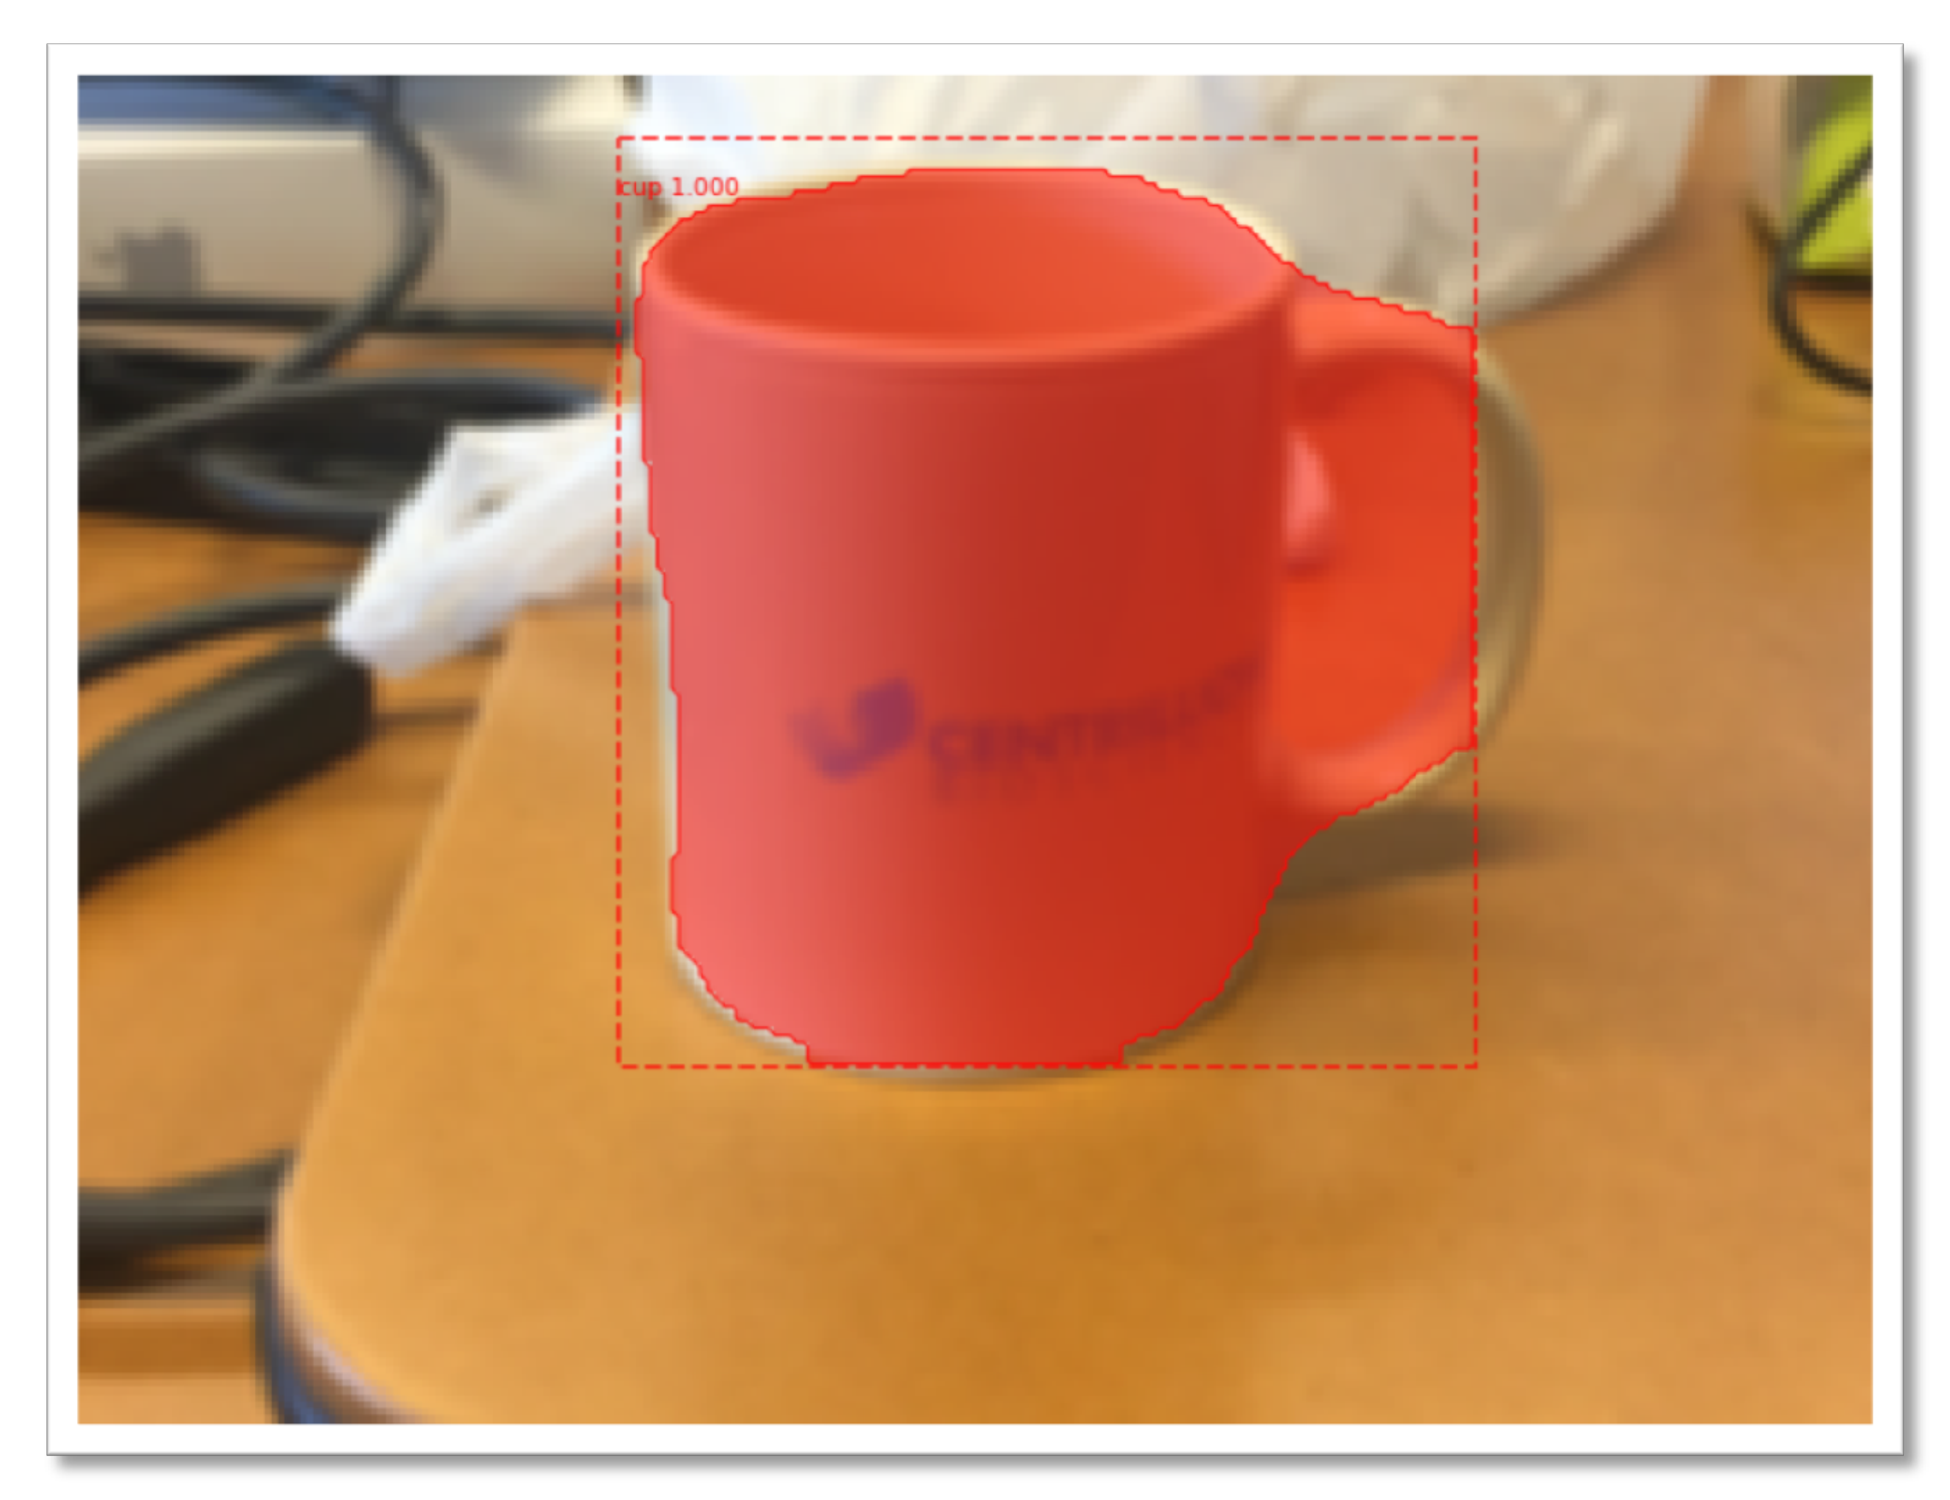
\includegraphics[width=.45\textwidth]{mask/mugori3}}%
	\hspace{2em}%
	\subcaptionbox{迁移学习后}
	{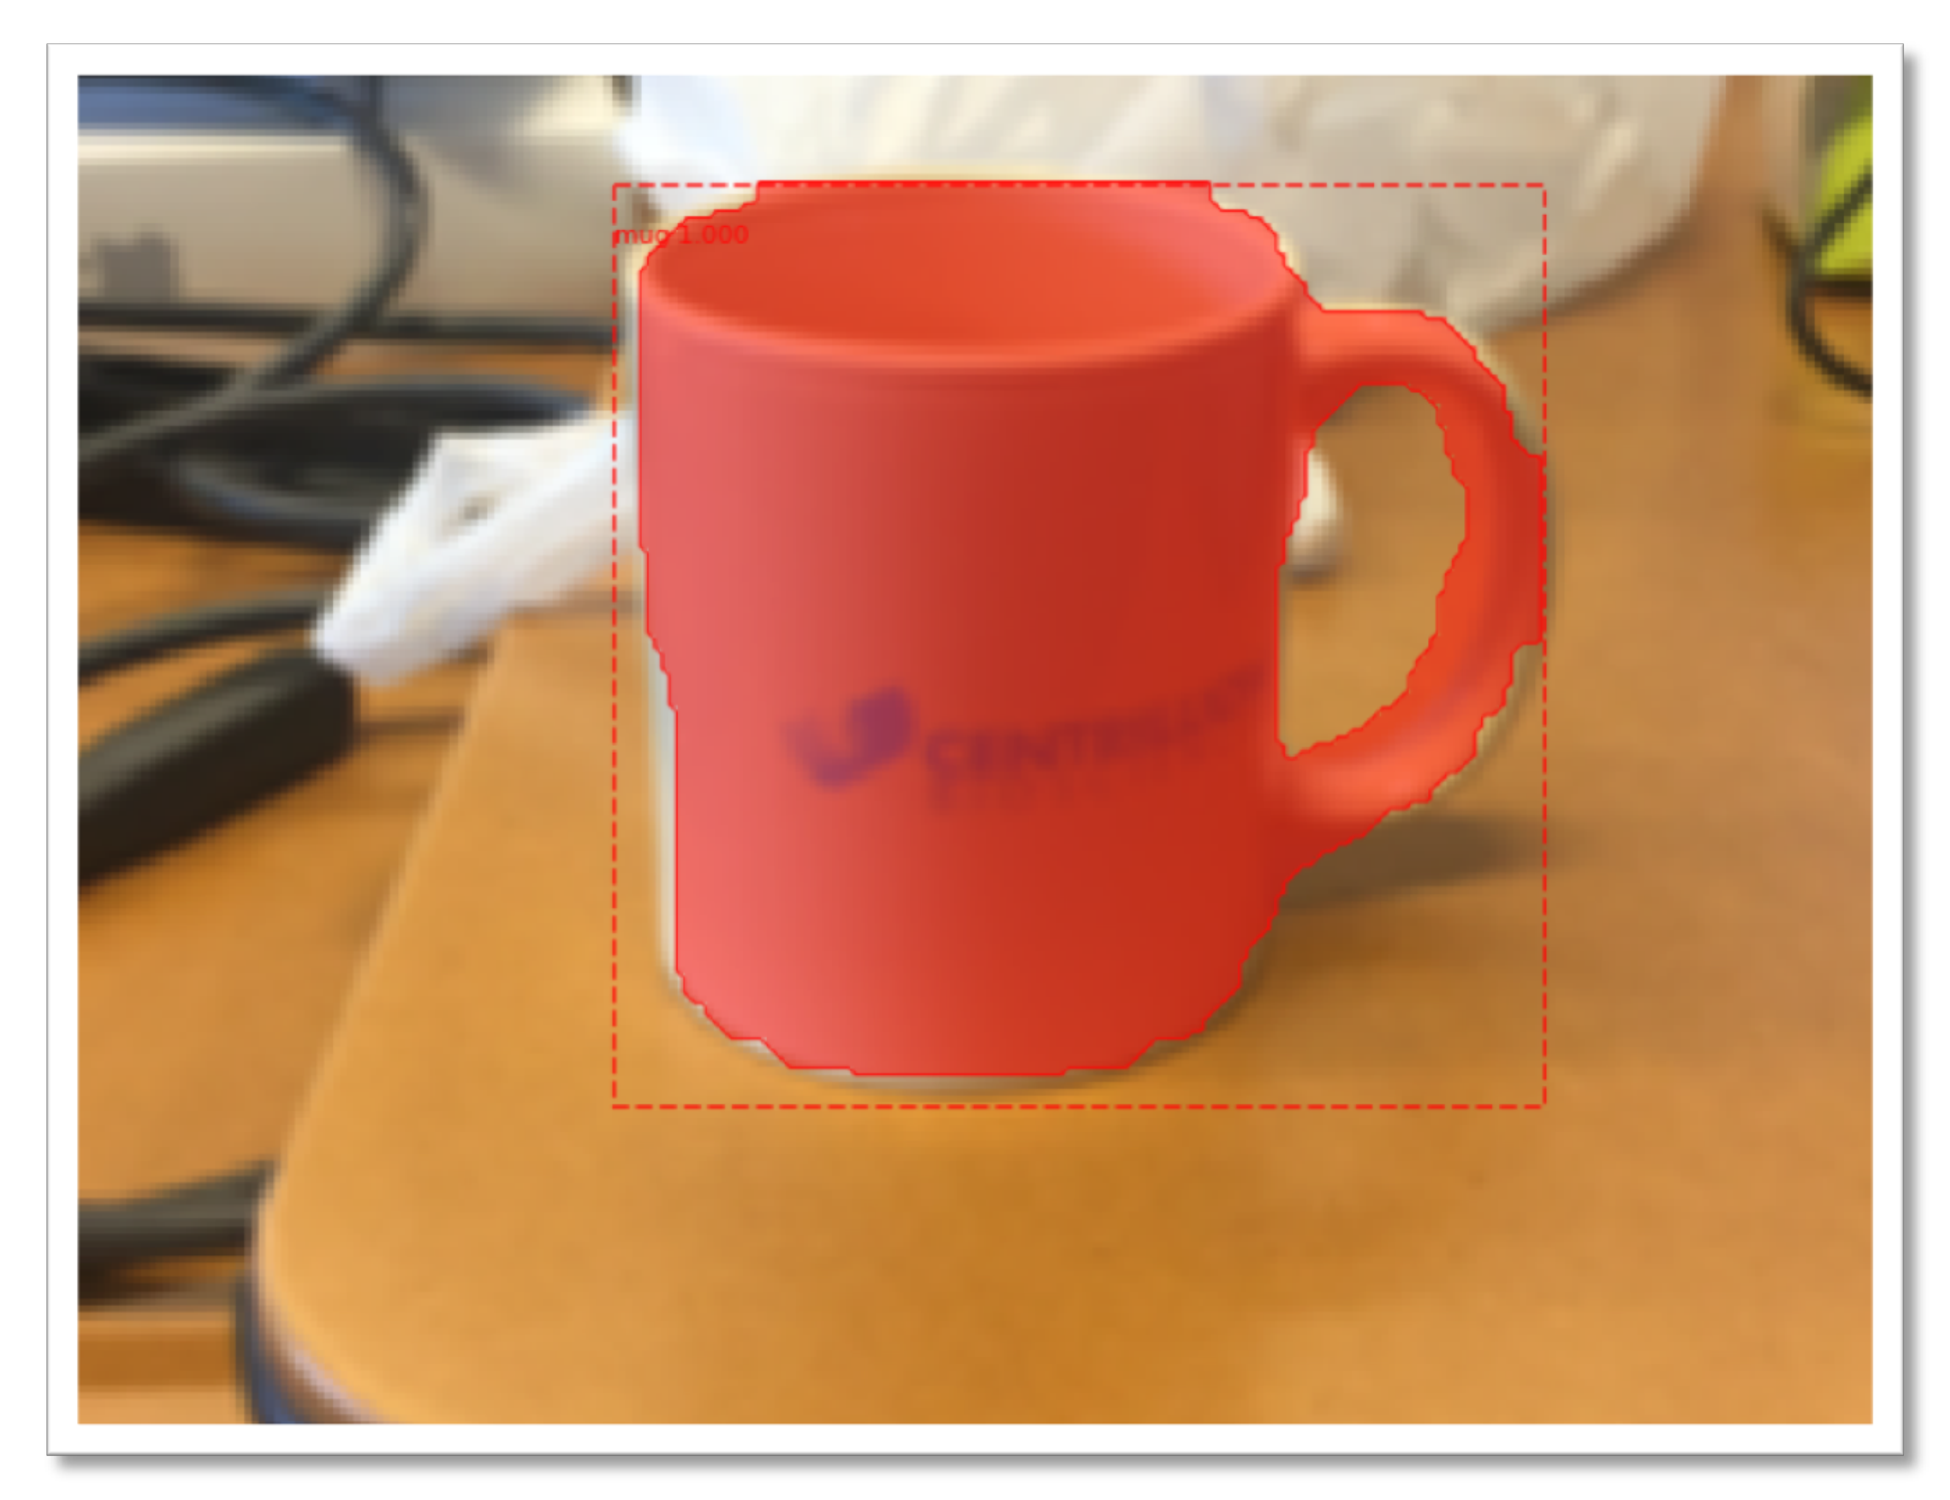
\includegraphics[width=.45\textwidth]{mask/mugreal3}}
	\caption{迁移学习对于 mask 的改善\label{fig:transferchange}}
\end{figure}

而迁移学习后的新网络在测试数据集上的表现 % 给出 Mask 
如图 \ref{fig:transfertest} 所示。
\begin{figure}[h]
	\centering%
	{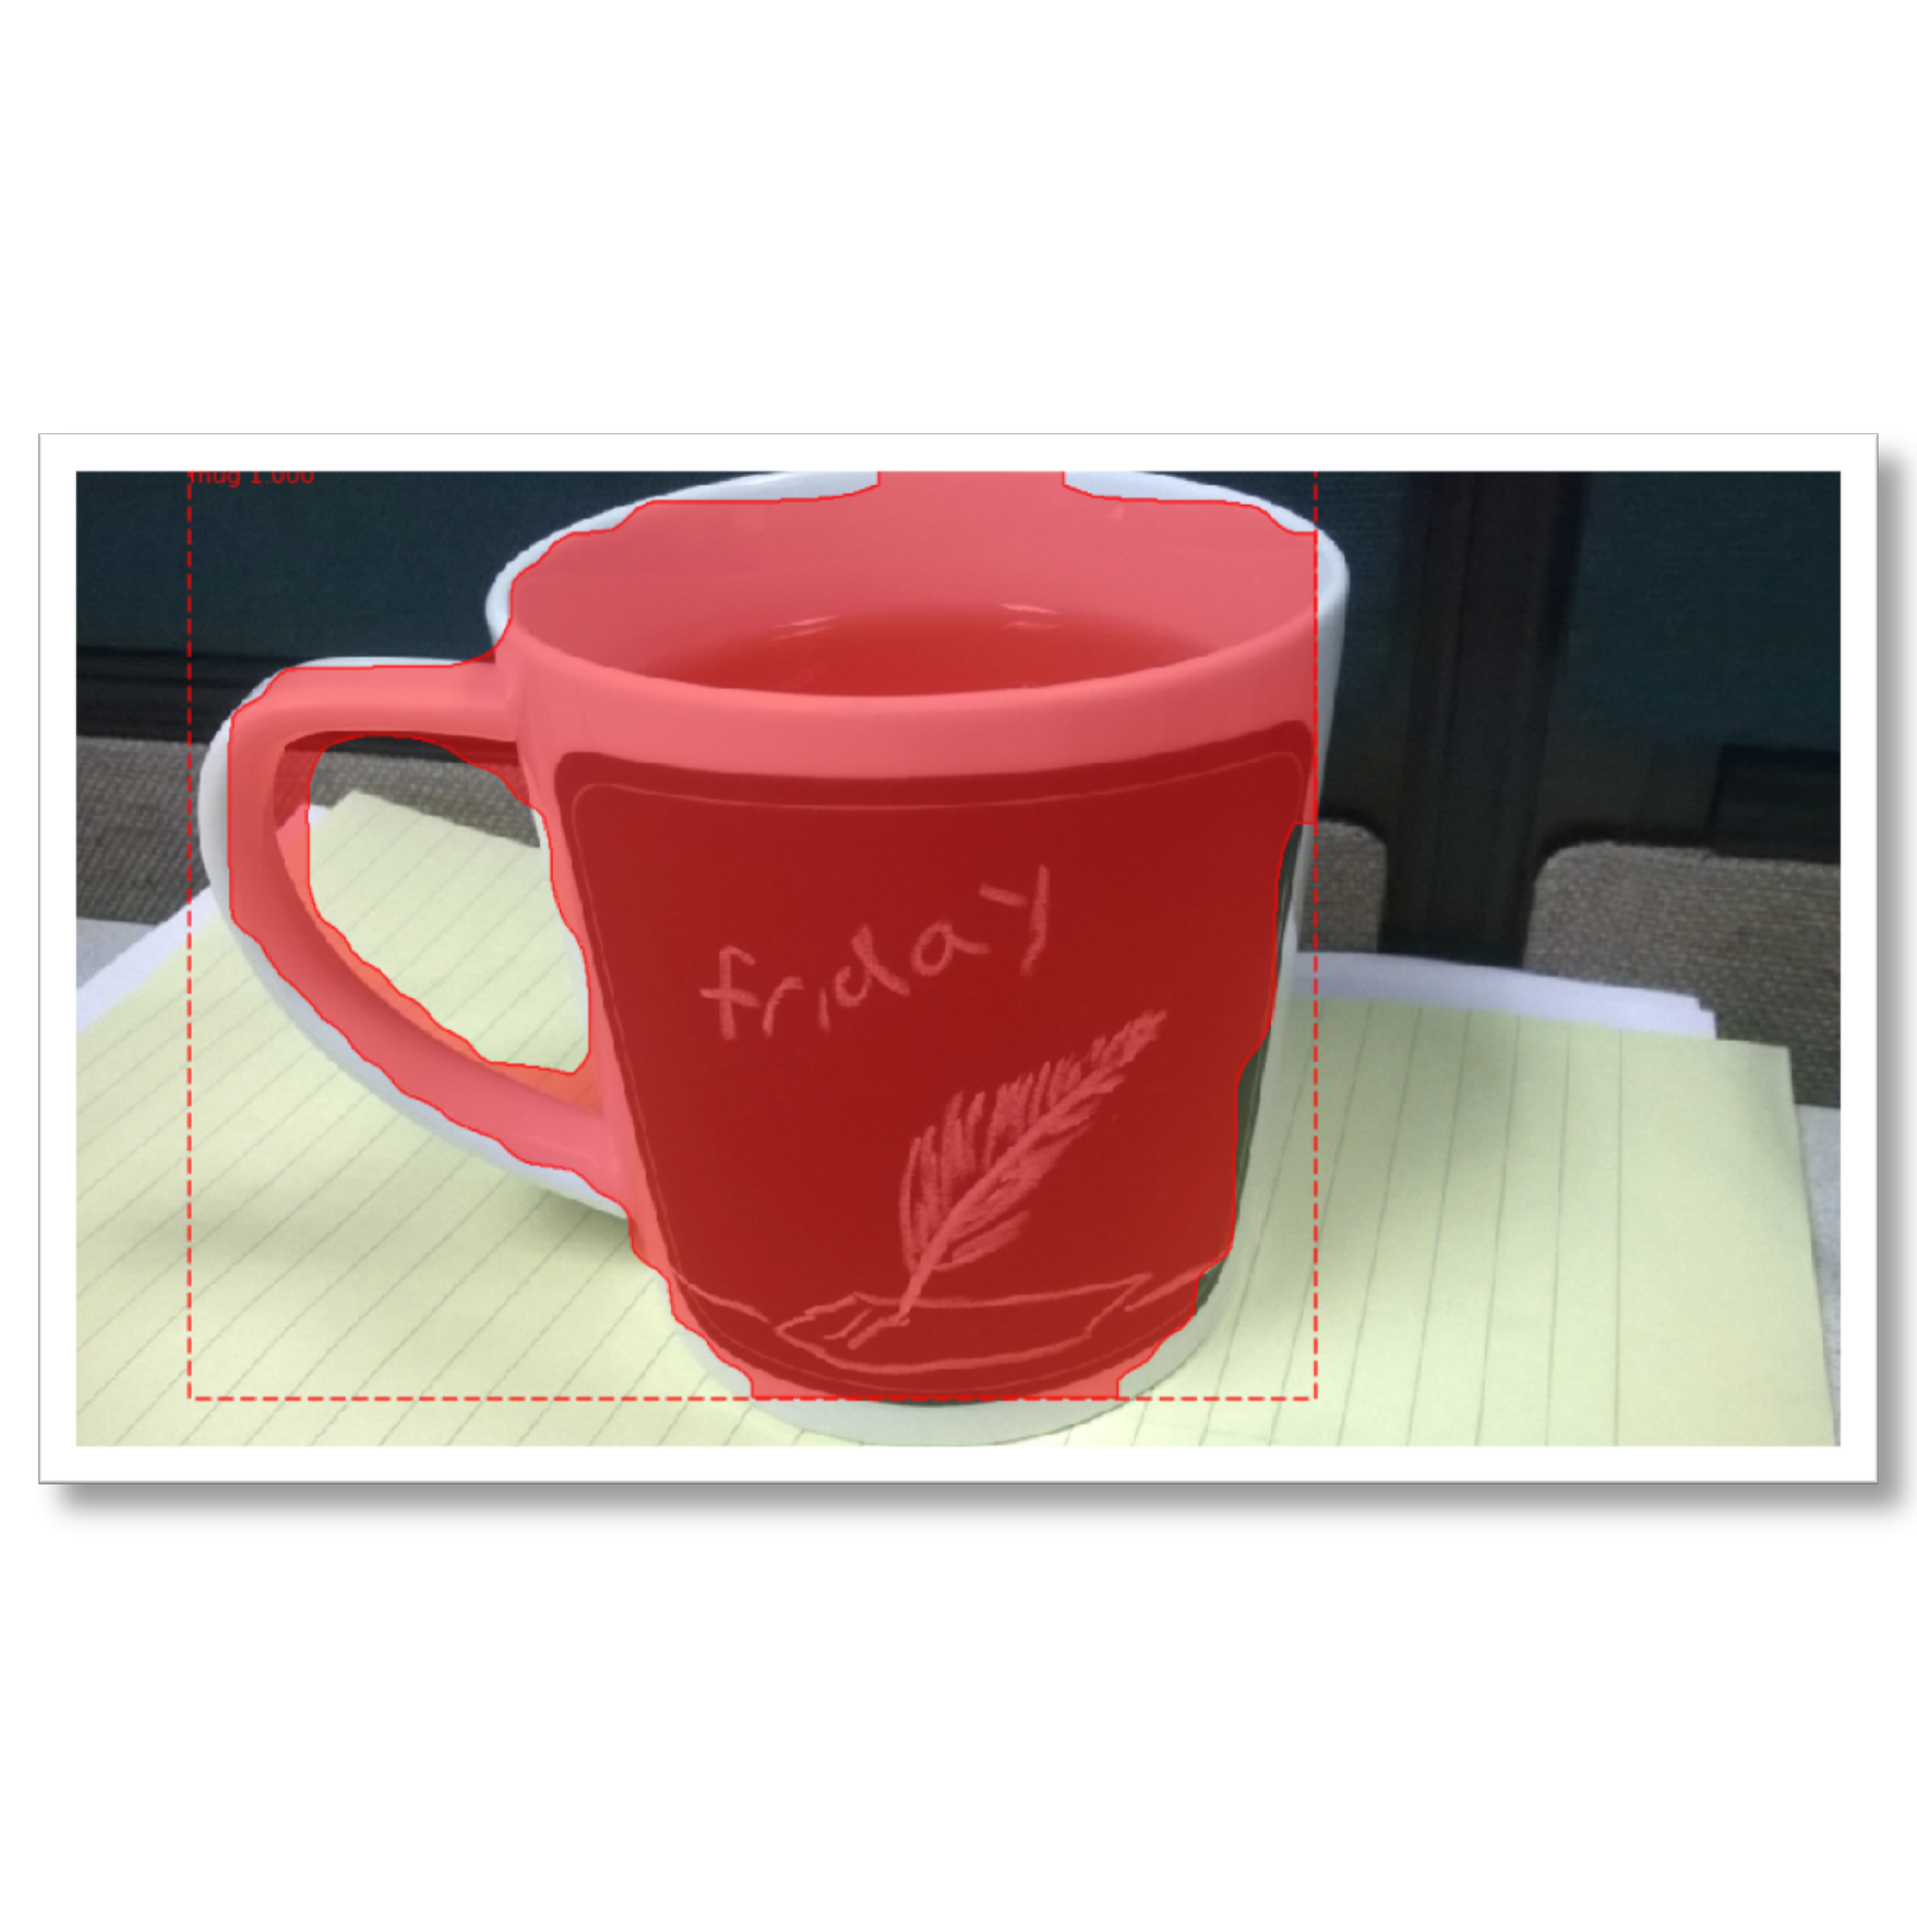
\includegraphics[width=.23\textwidth]{mask/mug1}}
	{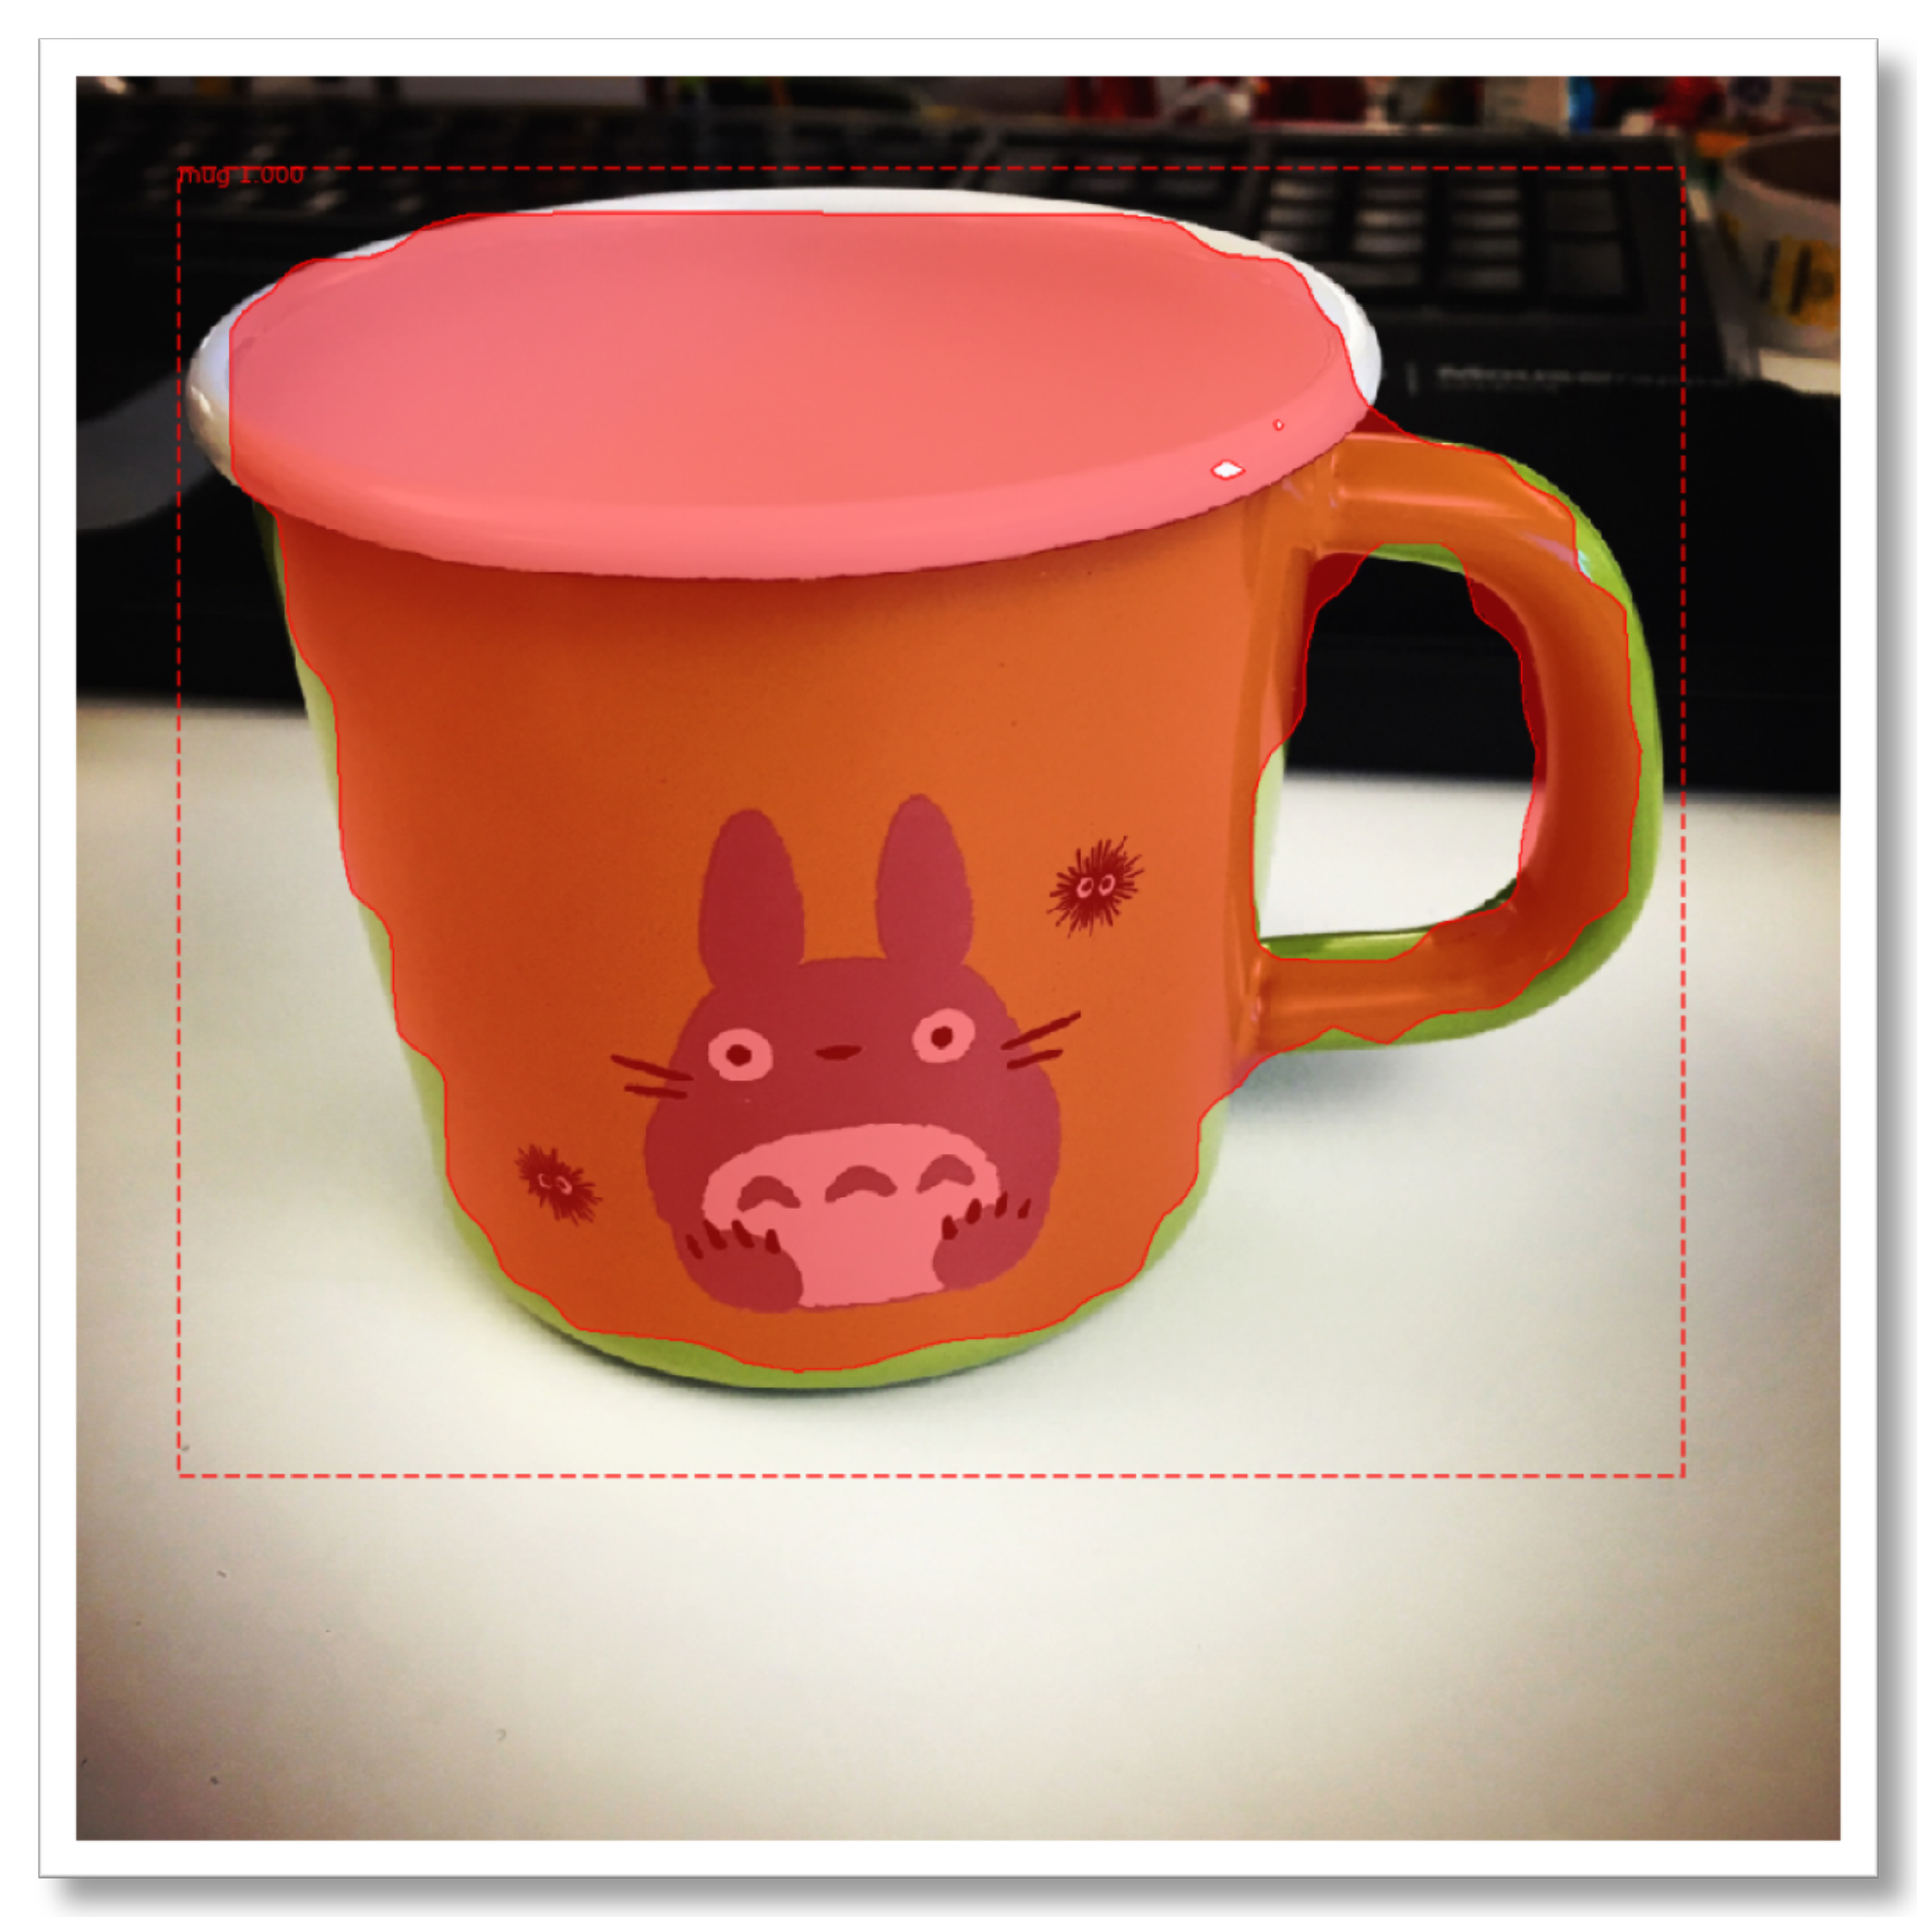
\includegraphics[width=.23\textwidth]{mask/mug2}}
	{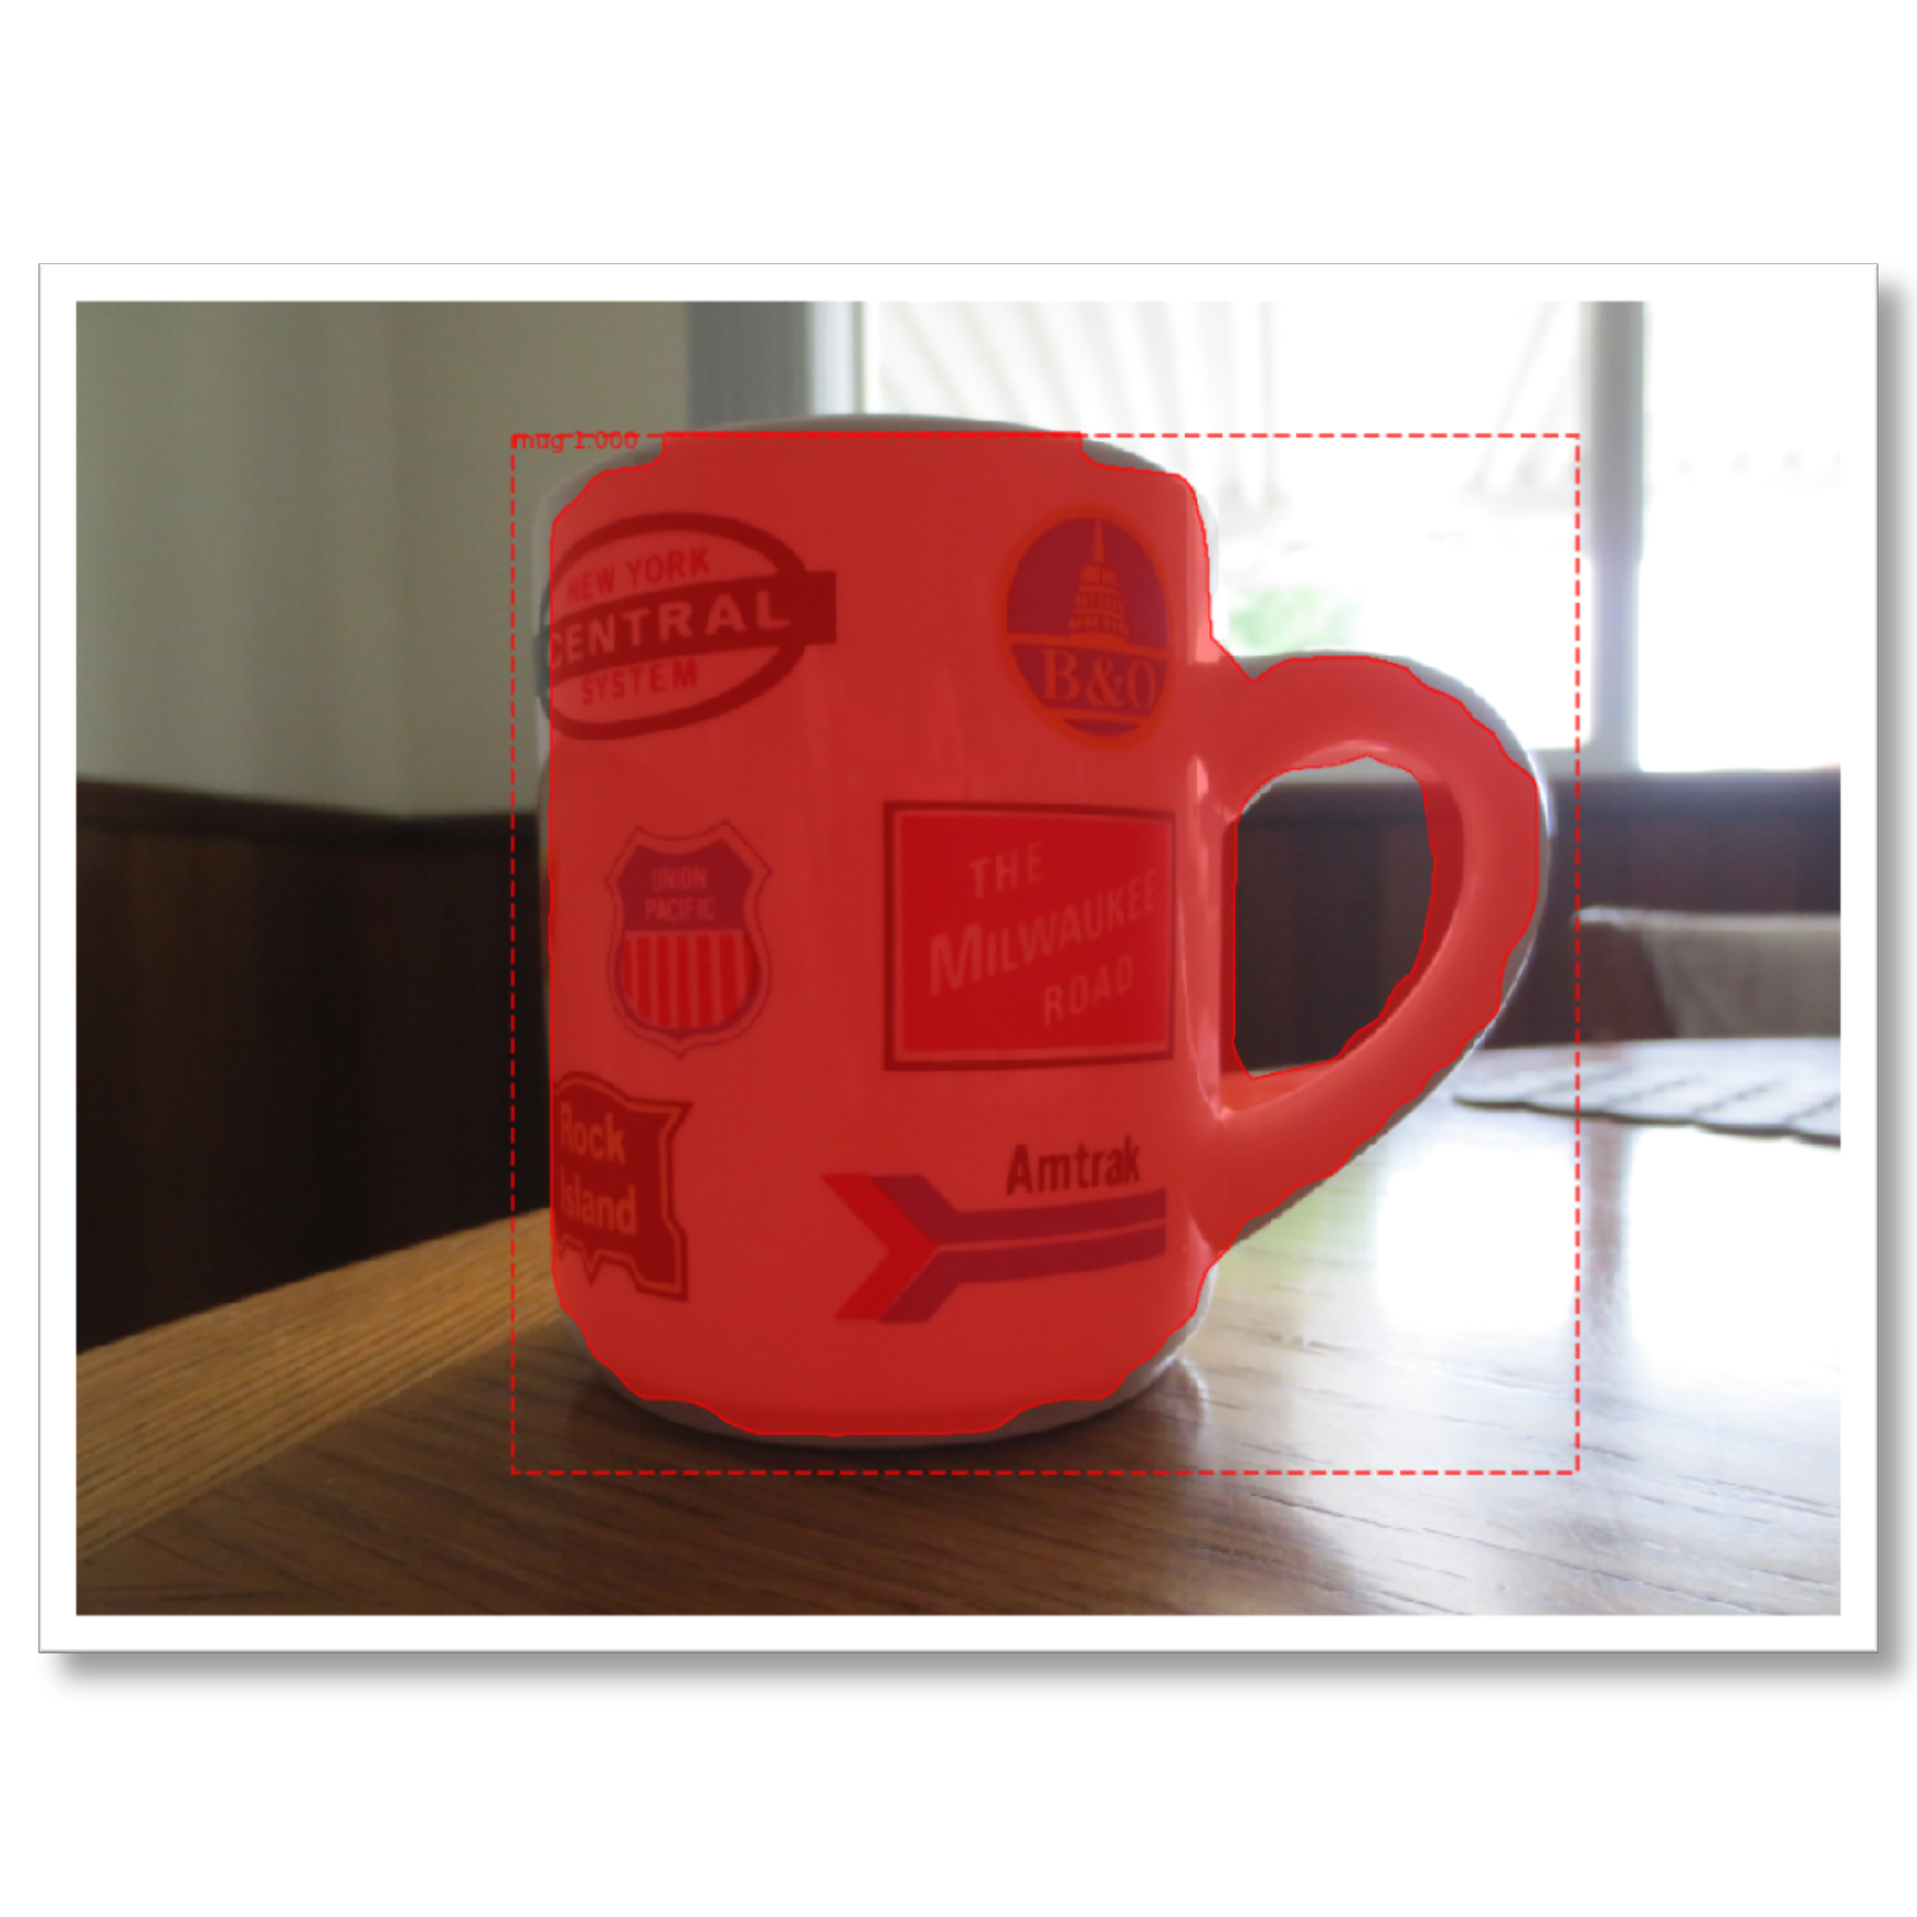
\includegraphics[width=.23\textwidth]{mask/mug3}}
	{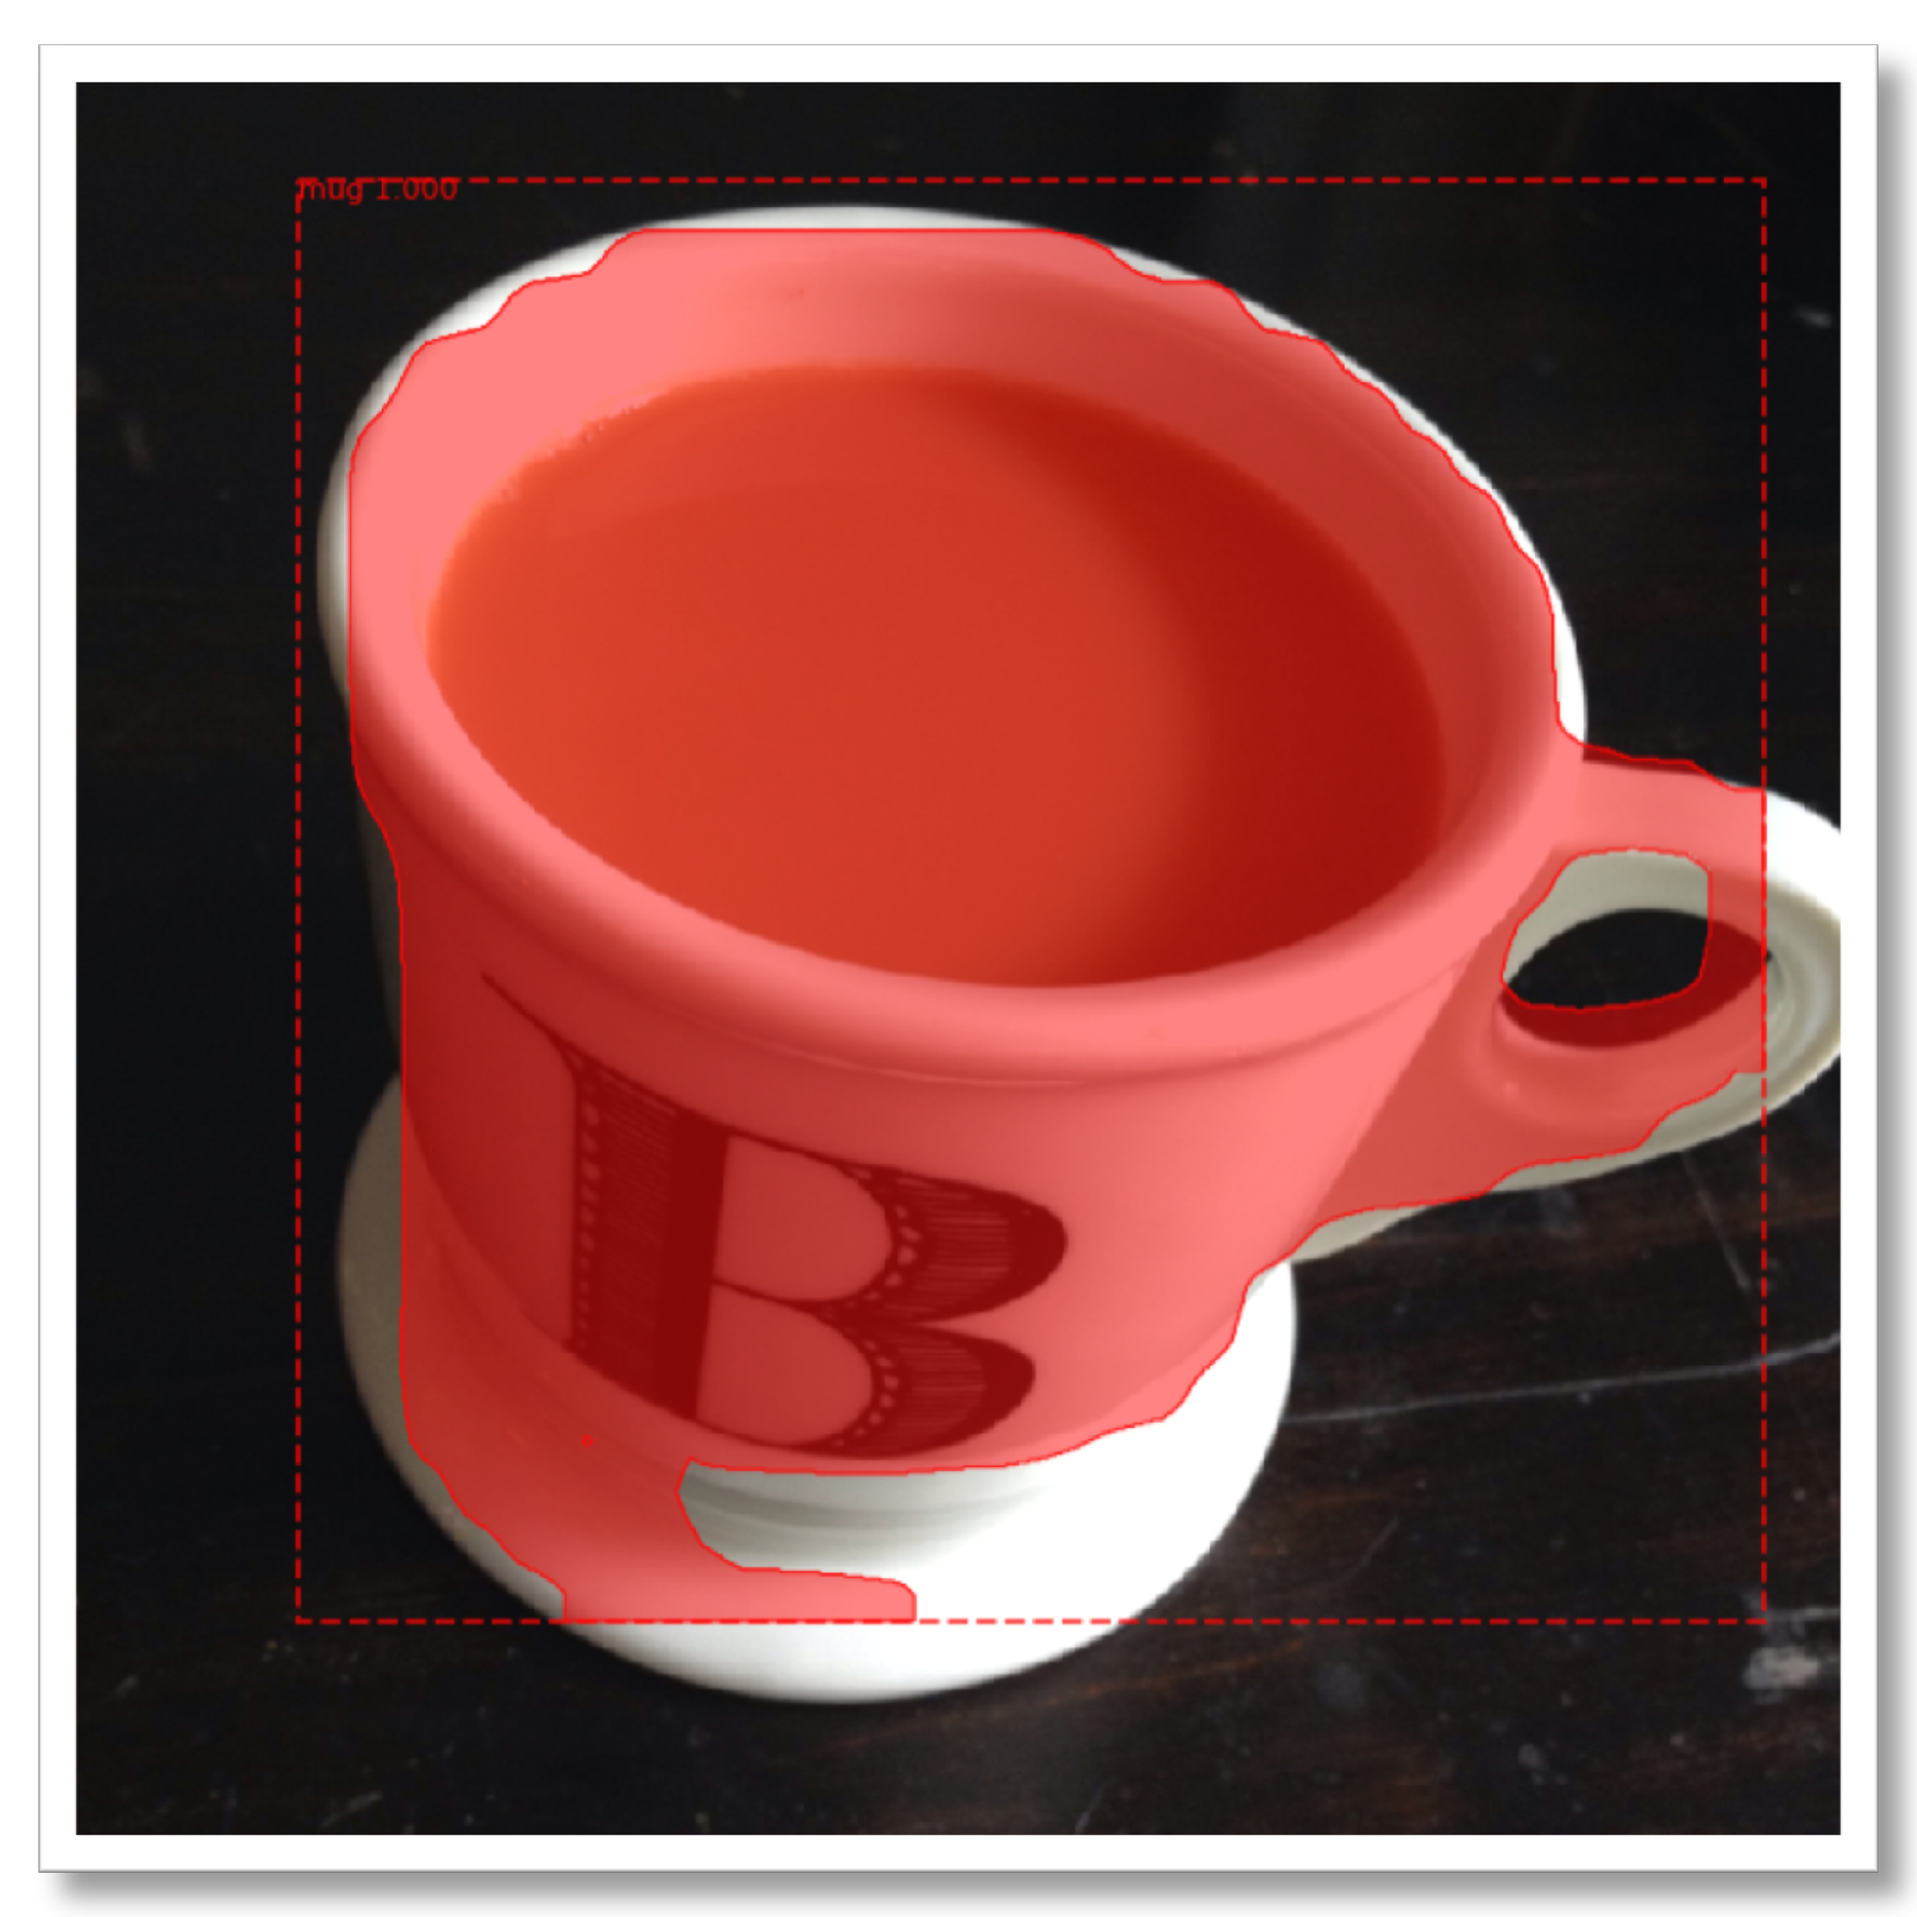
\includegraphics[width=.23\textwidth]{mask/mug4}}
	\caption{迁移学习后的 Mask R-CNN \cite{maskrcnn} 在测试集上的表现\label{fig:transfertest}}
\end{figure}

虽然我们没有在更多的类别上进行更广泛的测试,但我们相信,在迁移学习的指引下,预训练的模型与后期新标注的数据必将相辅相成,共同促进 mask 的质量%一定可以得到
的进一步提升。

% 重建表现

\subsection{三维重建 \label{section:recon}}

\newcounter{themenumber}
\newcounter{themenumber2}

我们首先使用 PointSetGen 工作的测试集,
对本工作和 PointSetGen 进行了实验,结果如表 \ref{tab:reconpsgdata} 所示。
对比两工作的重建结果,我们发现:虽然 PointSetGen 在原有的数据集上的重建结果尚可,%还可以被接受,
但本工作重建出的点云更稠密,更完整,而且对于几何形状的把握也明显的优于 PointSetGen。


\begin{longtable}[c]{c*{5}{c}}
	\caption{
		PointSetGen\cite{pointsetgen} 与本工作在 PointSetGen 测试集上的表现(部分)\label{tab:reconpsgdata}}                                      \\

	\toprule[1.5pt]
	{输入 $\bm I$}                                                                       & {\heiti 本工作} & {\heiti PSG\cite{pointsetgen}} &
	{输入 $\bm I$}                                                                       & {\heiti 本工作} & {\heiti PSG\cite{pointsetgen}}
	\\\midrule[1pt]
	\endfirsthead
	\multicolumn{6}{c}{续表~\thetable \hskip1em
		PointSetGen\cite{pointsetgen} 与本工作在 PointSetGen 测试集上的表现(部分)}                                                              \\
	\toprule[1.5pt]
	{输入 $\bm I$}                                                                       & {\heiti 本工作} & {\heiti PSG\cite{pointsetgen}} &
	{输入 $\bm I$}                                                                       & {\heiti 本工作} & {\heiti PSG\cite{pointsetgen}}
	\\\midrule[1pt]

	\endhead
	\bottomrule[1.5pt] %\hline
	\multicolumn{6}{r}{续下页}
	\endfoot
	\endlastfoot
	\forloop[2]{themenumber}{0}{\value{themenumber} < 32}
	{
		\setcounter{themenumber2}{\value{themenumber}}\addtocounter{themenumber2}{1}

	{\includegraphics[width=.14\textwidth]{cmp_psgdata/chair_\arabic{themenumber}}}      &
	{\includegraphics[width=.14\textwidth]{cmp_psgdata/our_chair_\arabic{themenumber}}}  &
	{\includegraphics[width=.14\textwidth]{cmp_psgdata/psg_chair_\arabic{themenumber}}}  &
	{\includegraphics[width=.14\textwidth]{cmp_psgdata/chair_\arabic{themenumber2}}}     &
	{\includegraphics[width=.14\textwidth]{cmp_psgdata/our_chair_\arabic{themenumber2}}} &
		{\includegraphics[width=.14\textwidth]{cmp_psgdata/psg_chair_\arabic{themenumber2}}}
		\\
	}

	\forloop[2]{themenumber}{0}{\value{themenumber} < 18}
	{
		\setcounter{themenumber2}{\value{themenumber}}\addtocounter{themenumber2}{1}

	{\includegraphics[width=.14\textwidth]{cmp_psgdata/car_\arabic{themenumber}}}        &
	{\includegraphics[width=.14\textwidth]{cmp_psgdata/our_car_\arabic{themenumber}}}    &
	{\includegraphics[width=.14\textwidth]{cmp_psgdata/psg_car_\arabic{themenumber}}}    &
	{\includegraphics[width=.14\textwidth]{cmp_psgdata/car_\arabic{themenumber2}}}       &
	{\includegraphics[width=.14\textwidth]{cmp_psgdata/our_car_\arabic{themenumber2}}}   &
		{\includegraphics[width=.14\textwidth]{cmp_psgdata/psg_car_\arabic{themenumber2}}}
		\\
	}

	\setcounter{themenumber2}{\value{themenumber}}\addtocounter{themenumber2}{1}

	{\includegraphics[width=.14\textwidth]{cmp_psgdata/car_\arabic{themenumber}}}        &
	{\includegraphics[width=.14\textwidth]{cmp_psgdata/our_car_\arabic{themenumber}}}    &
	{\includegraphics[width=.14\textwidth]{cmp_psgdata/psg_car_\arabic{themenumber}}}    &
	{\includegraphics[width=.14\textwidth]{cmp_psgdata/car_\arabic{themenumber2}}}       &
	{\includegraphics[width=.14\textwidth]{cmp_psgdata/our_car_\arabic{themenumber2}}}   &
	{\includegraphics[width=.14\textwidth]{cmp_psgdata/psg_car_\arabic{themenumber2}}}

	\\
	\bottomrule[1.5pt]
\end{longtable}







随后,我们还使用了本文的测试数据集,对两工作进行了测试,如表 \ref{tab:recon} 所示。
% 使用了第 \ref{section:mypre} 节中
% 介绍的增强数据集 %新数据集
% 详细讨论过
% 介绍的
% 增强数据集,取出其测试集,对两工作进行测试,如表 \ref{tab:recon} 所示。
%上 %中的测试集上
对比 PointSetGen 和本工作的重建结果,我们可以明显地看到 PointSetGen 在新数据上的表现很差,
因为训练 PointSetGen 所使用的训练数据集有缺陷,我们在第 \ref{section:mypre} 节中已有所提及。
而在本工作中,我们不仅使用了 VAE/GAN 保证了其重建质量
,还使用了增强后的新数据集进行训练,大大提高了网络的泛化能力,因此重建质量要明显优于 PointSetGen。


\begin{longtable}[c]{c*{5}{c}}
	\caption{
		PointSetGen\cite{pointsetgen} 与 本工作 在 本文测试集上的表现(部分)\label{tab:recon}}                                           \\

	\toprule[1.5pt]
	{输入 $\bm I$}                                                               & {\heiti 本工作} & {\heiti PSG\cite{pointsetgen}} &
	{输入 $\bm I$}                                                               & {\heiti 本工作} & {\heiti PSG\cite{pointsetgen}}
	\\\midrule[1pt]
	\endfirsthead
	\multicolumn{6}{c}{续表~\thetable \hskip1em
		PointSetGen\cite{pointsetgen}  与 本工作 在 本文测试集上的表现(部分)}                                                           \\
	\toprule[1.5pt]
	{输入 $\bm I$}                                                               & {\heiti 本工作} & {\heiti PSG\cite{pointsetgen}} &
	{输入 $\bm I$}                                                               & {\heiti 本工作} & {\heiti PSG\cite{pointsetgen}}
	\\\midrule[1pt]


	\endhead
	\bottomrule[1.5pt] %\hline
	\multicolumn{6}{r}{续下页}
	\endfoot
	\endlastfoot
	% \forloop{themenumber}{1}{\value{themenumber} < 31}
	% {
	% {\includegraphics[width=.14\textwidth]{cmp/car_\arabic{themenumber}}}&
	% {\includegraphics[width=.14\textwidth]{cmp/our_car_\arabic{themenumber}}}&
	% {\includegraphics[width=.14\textwidth]{cmp/psg_car_\arabic{themenumber}}}&
	% {\includegraphics[width=.14\textwidth]{cmp/chair_\arabic{themenumber}}}&
	% {\includegraphics[width=.14\textwidth]{cmp/our_chair_\arabic{themenumber}}}&
	% {\includegraphics[width=.14\textwidth]{cmp/psg_chair_\arabic{themenumber}}}
	% \\
	% }
	% {\includegraphics[width=.14\textwidth]{cmp/car_\arabic{themenumber}}}&
	% {\includegraphics[width=.14\textwidth]{cmp/our_car_\arabic{themenumber}}}&
	% {\includegraphics[width=.14\textwidth]{cmp/psg_car_\arabic{themenumber}}}&
	% {\includegraphics[width=.14\textwidth]{cmp/chair_\arabic{themenumber}}}&
	% {\includegraphics[width=.14\textwidth]{cmp/our_chair_\arabic{themenumber}}}&
	% {\includegraphics[width=.14\textwidth]{cmp/psg_chair_\arabic{themenumber}}}
	% \\
	\forloop[2]{themenumber}{0}{\value{themenumber} < 32}
	{
		\setcounter{themenumber2}{\value{themenumber}}\addtocounter{themenumber2}{1}

	{\includegraphics[width=.14\textwidth]{cmp/chair_\arabic{themenumber}}}      &
	{\includegraphics[width=.14\textwidth]{cmp/our_chair_\arabic{themenumber}}}  &
	{\includegraphics[width=.14\textwidth]{cmp/psg_chair_\arabic{themenumber}}}  &
	{\includegraphics[width=.14\textwidth]{cmp/chair_\arabic{themenumber2}}}     &
	{\includegraphics[width=.14\textwidth]{cmp/our_chair_\arabic{themenumber2}}} &
		{\includegraphics[width=.14\textwidth]{cmp/psg_chair_\arabic{themenumber2}}}
		\\
	}
	\forloop[2]{themenumber}{0}{\value{themenumber} < 30}
	{
		\setcounter{themenumber2}{\value{themenumber}}\addtocounter{themenumber2}{1}

	{\includegraphics[width=.14\textwidth]{cmp/car_\arabic{themenumber}}}        &
	{\includegraphics[width=.14\textwidth]{cmp/our_car_\arabic{themenumber}}}    &
	{\includegraphics[width=.14\textwidth]{cmp/psg_car_\arabic{themenumber}}}    &
	{\includegraphics[width=.14\textwidth]{cmp/car_\arabic{themenumber2}}}       &
	{\includegraphics[width=.14\textwidth]{cmp/our_car_\arabic{themenumber2}}}   &
		{\includegraphics[width=.14\textwidth]{cmp/psg_car_\arabic{themenumber2}}}
		\\
	}
	\setcounter{themenumber2}{\value{themenumber}}\addtocounter{themenumber2}{1}

	{\includegraphics[width=.14\textwidth]{cmp/car_\arabic{themenumber}}}        &
	{\includegraphics[width=.14\textwidth]{cmp/our_car_\arabic{themenumber}}}    &
	{\includegraphics[width=.14\textwidth]{cmp/psg_car_\arabic{themenumber}}}    &
	{\includegraphics[width=.14\textwidth]{cmp/car_\arabic{themenumber2}}}       &
	{\includegraphics[width=.14\textwidth]{cmp/our_car_\arabic{themenumber2}}}   &
	{\includegraphics[width=.14\textwidth]{cmp/psg_car_\arabic{themenumber2}}}
	\\
	\bottomrule[1.5pt]
\end{longtable}






此外,我们还测试了从真实照片中重建的情况,如表 \ref{tab:realimg} 所示。

\begin{longtable}[c]{c*{2}{c}}
	\caption{
		PointSetGen\cite{pointsetgen} 与 本工作 在真实照片中的表现(部分)\label{tab:realimg}}                     \\
	\toprule[1.5pt]
	{输入 $\bm I$}                                          & {\heiti 本工作} & {\heiti PSG\cite{pointsetgen}}
	\\\midrule[1pt]
	\endfirsthead
	\multicolumn{3}{c}{续表~\thetable \hskip1em
		PointSetGen\cite{pointsetgen} 与 本工作 在真实照片中的表现(部分)}                                        \\
	\toprule[1.5pt]
	{输入 $\bm I$}                                          & {\heiti 本工作} & {\heiti PSG\cite{pointsetgen}}
	\\\midrule[1pt]
	\endhead
	\bottomrule[1.5pt] %\hline
	\multicolumn{3}{r}{续下页}
	\endfoot
	\endlastfoot

	{\includegraphics[width=.32\textwidth]{cmp/car1}}       &
	{\includegraphics[width=.32\textwidth]{cmp/car1_our}}   &
	{\includegraphics[width=.32\textwidth]{cmp/car1_psg}}
	\\
	{\includegraphics[width=.30\textwidth]{cmp/car2}}       &
	{\includegraphics[width=.30\textwidth]{cmp/car2_our}}   &
	{\includegraphics[width=.30\textwidth]{cmp/car2_psg}}
	\\
	{\includegraphics[width=.30\textwidth]{cmp/car3}}       &
	{\includegraphics[width=.30\textwidth]{cmp/car3_our}}   &
	{\includegraphics[width=.30\textwidth]{cmp/car3_psg}}
	\\
	{\includegraphics[width=.30\textwidth]{cmp/chair1}}     &
	{\includegraphics[width=.30\textwidth]{cmp/chair1_our}} &
	{\includegraphics[width=.30\textwidth]{cmp/chair1_psg}}
	\\
	{\includegraphics[width=.30\textwidth]{cmp/chair2}}     &
	{\includegraphics[width=.30\textwidth]{cmp/chair2_our}} &
	{\includegraphics[width=.30\textwidth]{cmp/chair2_psg}}
	\\
	{\includegraphics[width=.30\textwidth]{cmp/chair6}}     &
	{\includegraphics[width=.30\textwidth]{cmp/chair6_our}} &
	{\includegraphics[width=.30\textwidth]{cmp/chair6_psg}}
	\\
	\bottomrule[1.5pt]
\end{longtable}

总体而言,无论是在%本文的
测试集上还是在真实照片上,本文工作的重建效果都要优于 PointSetGen。因此,我们曾在第 \ref{section:myquestion} 节中提出的增强重建效果的目标已经基本实现。
% 插值表现

% 算术表现

\subsection{插值表现}



由于我们采用了 VAE/GAN 结构,因此我们可以按照用户的需求,对于生成的结果进行插值,以改进用户对于系统的可控性。
这是 PointSetGen 所不能实现的功能,也是本文工作的优势之一。

表 \ref{tab:inter} 展示了一个对
%表 \ref{tab:realimg} 中
第 \ref{section:recon} 节中的重建结果进行插值的例子。

\begin{longtable}[c]{c*{5}{c}}
	\caption{本工作对于重建结果插值的表现 \label{tab:inter}}                                               \\

	\toprule[1.5pt]
	{输入 $\bm I_1$}                                                & {\heiti 插值结果} & {输入 $\bm I_2$}
	\\\midrule[1pt]

	\endfirsthead
	\multicolumn{3}{c}{续表~\thetable \hskip1em  本工作对于重建结果插值的表现}                             \\

	\toprule[1.5pt]
	{输入 $\bm I_1$}                                                & {\heiti 插值结果} & {输入 $\bm I_2$}
	\\\midrule[1pt]

	\endhead
	\bottomrule[1.5pt] %\hline
	\multicolumn{3}{r}{续下页}
	\endfoot
	\endlastfoot
	{\includegraphics[width=.12\textwidth]{cmp/chair2}}             &
	{\includegraphics[width=.12\textwidth]{inter/chair_12_0100000}}
		{\includegraphics[width=.12\textwidth]{inter/chair_12_0300000}}
		{\includegraphics[width=.12\textwidth]{inter/chair_12_0500000}}
		{\includegraphics[width=.12\textwidth]{inter/chair_12_0700000}}
	{\includegraphics[width=.12\textwidth]{inter/chair_12_0900000}} &
	{\includegraphics[width=.12\textwidth]{cmp/chair1}}
	\\
	{\includegraphics[width=.12\textwidth]{cmp/chair6}}             &
	{\includegraphics[width=.12\textwidth]{inter/chair_26_0100000}}
		{\includegraphics[width=.12\textwidth]{inter/chair_26_0300000}}
		{\includegraphics[width=.12\textwidth]{inter/chair_26_0500000}}
		{\includegraphics[width=.12\textwidth]{inter/chair_26_0700000}}
	{\includegraphics[width=.12\textwidth]{inter/chair_26_0900000}} &
	{\includegraphics[width=.12\textwidth]{cmp/chair2}}
	\\
	{\includegraphics[width=.12\textwidth]{cmp/chair1}}             &
	{\includegraphics[width=.12\textwidth]{inter/chair_61_0100000}}
		{\includegraphics[width=.12\textwidth]{inter/chair_61_0300000}}
		{\includegraphics[width=.12\textwidth]{inter/chair_61_0500000}}
		{\includegraphics[width=.12\textwidth]{inter/chair_61_0700000}}
	{\includegraphics[width=.12\textwidth]{inter/chair_61_0900000}} &
	{\includegraphics[width=.12\textwidth]{cmp/chair6}}
	\\

	{\includegraphics[width=.12\textwidth]{cmp/car2}}               &
	{\includegraphics[width=.12\textwidth]{inter/car_12_0100000}}
		{\includegraphics[width=.12\textwidth]{inter/car_12_0300000}}
		{\includegraphics[width=.12\textwidth]{inter/car_12_0500000}}
		{\includegraphics[width=.12\textwidth]{inter/car_12_0700000}}
	{\includegraphics[width=.12\textwidth]{inter/car_12_0900000}}   &
	{\includegraphics[width=.12\textwidth]{cmp/car1}}
	\\
	{\includegraphics[width=.12\textwidth]{cmp/car3}}               &
	{\includegraphics[width=.12\textwidth]{inter/car_23_0100000}}
		{\includegraphics[width=.12\textwidth]{inter/car_23_0300000}}
		{\includegraphics[width=.12\textwidth]{inter/car_23_0500000}}
		{\includegraphics[width=.12\textwidth]{inter/car_23_0700000}}
	{\includegraphics[width=.12\textwidth]{inter/car_23_0900000}}   &
	{\includegraphics[width=.12\textwidth]{cmp/car2}}
	\\
	{\includegraphics[width=.12\textwidth]{cmp/car1}}               &
	{\includegraphics[width=.12\textwidth]{inter/car_31_0100000}}
		{\includegraphics[width=.12\textwidth]{inter/car_31_0300000}}
		{\includegraphics[width=.12\textwidth]{inter/car_31_0500000}}
		{\includegraphics[width=.12\textwidth]{inter/car_31_0700000}}
	{\includegraphics[width=.12\textwidth]{inter/car_31_0900000}}   &
	{\includegraphics[width=.12\textwidth]{cmp/car3}}
	\\
	\bottomrule[1.5pt]
\end{longtable}


\section{流水线架构}
将第 \ref{section:mask}、 \ref{section:recon} 节中介绍的 mask 提取算法和重建算法结合,就形成了本文的流水线架构,如图 \ref{fig:mypipeline} 所示。

\begin{figure}[h]
	\centering%
	\subcaptionbox{输入图像}
	{\includegraphics[width=.30\textwidth]{pipe1}}%
	\hspace{1em}%
	\subcaptionbox{mask 生成}
	{\includegraphics[width=.30\textwidth]{pipe2}}
	\hspace{1em}%
	\subcaptionbox{重建输出}
	{\includegraphics[width=.30\textwidth]{pipe3}}
	\caption{本工作的流水线架构 \label{fig:mypipeline}}
\end{figure}


可以看到,这两个算法协同运作、相辅相成,
共同解决了基于单张 RGB 图像的
三维物体点云重建任务。重建结果表明,本工作已经达到了第 \ref{section:myquestion} 节中提出的基本要求与预期目标。

%,且重建结果的质量依然有所保障。
% 它们,共同组成了本文的主算法。